\documentclass{acm_proc_article-sp}
\usepackage[utf8]{inputenc}

\renewcommand{\paragraph}[1]{\vskip 6pt\noindent\textbf{#1 }}
\usepackage{hyperref}
\usepackage{graphicx}
\usepackage{url}

\providecommand{\tightlist}{%
  \setlength{\itemsep}{0pt}\setlength{\parskip}{0pt}}

\title{Realis Guru - The One-Stop Help for HDB Buyers \& Sellers}


% Add imagehandling
\usepackage{graphicx}
% Redefine \includegraphics so that, unless explicit options are
% given, the image width will not exceed the width of the page.
% Images get their normal width if they fit onto the page, but
% are scaled down if they would overflow the margins.
\makeatletter
\def\ScaleIfNeeded{%
  \ifdim\Gin@nat@width>\linewidth
    \linewidth
  \else
    \Gin@nat@width
  \fi
}
\makeatother
\let\Oldincludegraphics\includegraphics
{%
 \catcode`\@=11\relax%
 \gdef\includegraphics{\@ifnextchar[{\Oldincludegraphics}{\Oldincludegraphics[width=\ScaleIfNeeded]}}%
}%

\numberofauthors{2}
\author{
\alignauthor Amrita Mishra \\
        \affaddr{Singapore Management University}\\
       \email{\href{mailto:amritam.2020@mitb.smu.edu.sg}{\nolinkurl{amritam.2020@mitb.smu.edu.sg}}}
\and \alignauthor Sng Kah Leong \\
        \affaddr{Singapore Management University}\\
       \email{\href{mailto:klsng.2020@mitb.smu.edu.sg}{\nolinkurl{klsng.2020@mitb.smu.edu.sg}}}
\and }

\date{}

%Remove copyright shit
\permission{}
\conferenceinfo{} {}
\CopyrightYear{}
\crdata{}

% Pandoc syntax highlighting
\usepackage{color}
\usepackage{fancyvrb}
\newcommand{\VerbBar}{|}
\newcommand{\VERB}{\Verb[commandchars=\\\{\}]}
\DefineVerbatimEnvironment{Highlighting}{Verbatim}{commandchars=\\\{\}}
% Add ',fontsize=\small' for more characters per line
\usepackage{framed}
\definecolor{shadecolor}{RGB}{248,248,248}
\newenvironment{Shaded}{\begin{snugshade}}{\end{snugshade}}
\newcommand{\AlertTok}[1]{\textcolor[rgb]{0.94,0.16,0.16}{#1}}
\newcommand{\AnnotationTok}[1]{\textcolor[rgb]{0.56,0.35,0.01}{\textbf{\textit{#1}}}}
\newcommand{\AttributeTok}[1]{\textcolor[rgb]{0.77,0.63,0.00}{#1}}
\newcommand{\BaseNTok}[1]{\textcolor[rgb]{0.00,0.00,0.81}{#1}}
\newcommand{\BuiltInTok}[1]{#1}
\newcommand{\CharTok}[1]{\textcolor[rgb]{0.31,0.60,0.02}{#1}}
\newcommand{\CommentTok}[1]{\textcolor[rgb]{0.56,0.35,0.01}{\textit{#1}}}
\newcommand{\CommentVarTok}[1]{\textcolor[rgb]{0.56,0.35,0.01}{\textbf{\textit{#1}}}}
\newcommand{\ConstantTok}[1]{\textcolor[rgb]{0.00,0.00,0.00}{#1}}
\newcommand{\ControlFlowTok}[1]{\textcolor[rgb]{0.13,0.29,0.53}{\textbf{#1}}}
\newcommand{\DataTypeTok}[1]{\textcolor[rgb]{0.13,0.29,0.53}{#1}}
\newcommand{\DecValTok}[1]{\textcolor[rgb]{0.00,0.00,0.81}{#1}}
\newcommand{\DocumentationTok}[1]{\textcolor[rgb]{0.56,0.35,0.01}{\textbf{\textit{#1}}}}
\newcommand{\ErrorTok}[1]{\textcolor[rgb]{0.64,0.00,0.00}{\textbf{#1}}}
\newcommand{\ExtensionTok}[1]{#1}
\newcommand{\FloatTok}[1]{\textcolor[rgb]{0.00,0.00,0.81}{#1}}
\newcommand{\FunctionTok}[1]{\textcolor[rgb]{0.00,0.00,0.00}{#1}}
\newcommand{\ImportTok}[1]{#1}
\newcommand{\InformationTok}[1]{\textcolor[rgb]{0.56,0.35,0.01}{\textbf{\textit{#1}}}}
\newcommand{\KeywordTok}[1]{\textcolor[rgb]{0.13,0.29,0.53}{\textbf{#1}}}
\newcommand{\NormalTok}[1]{#1}
\newcommand{\OperatorTok}[1]{\textcolor[rgb]{0.81,0.36,0.00}{\textbf{#1}}}
\newcommand{\OtherTok}[1]{\textcolor[rgb]{0.56,0.35,0.01}{#1}}
\newcommand{\PreprocessorTok}[1]{\textcolor[rgb]{0.56,0.35,0.01}{\textit{#1}}}
\newcommand{\RegionMarkerTok}[1]{#1}
\newcommand{\SpecialCharTok}[1]{\textcolor[rgb]{0.00,0.00,0.00}{#1}}
\newcommand{\SpecialStringTok}[1]{\textcolor[rgb]{0.31,0.60,0.02}{#1}}
\newcommand{\StringTok}[1]{\textcolor[rgb]{0.31,0.60,0.02}{#1}}
\newcommand{\VariableTok}[1]{\textcolor[rgb]{0.00,0.00,0.00}{#1}}
\newcommand{\VerbatimStringTok}[1]{\textcolor[rgb]{0.31,0.60,0.02}{#1}}
\newcommand{\WarningTok}[1]{\textcolor[rgb]{0.56,0.35,0.01}{\textbf{\textit{#1}}}}

% Pandoc citation processing


\begin{document}
\maketitle

\begin{abstract}
Singapore is a small country with limited land resources to convert into
housing. With a growing population need to meet the aggressive economic
demands, Singapore Government is encouraging current residents to have
more children while simultaneously importing niche and raw talent from
other countries to set up their base here. This is increasing the demand
for both public and private housing. Public housing (also known as HDB)
is subsidized by the government to give the citizens an opportunity to
make their own homes at a lower cost.

While HDB website has some of the historical data, it does not have a 1
stop view of the island wide statistics. Through our R Shiny
application, we hope to provide our users an interactive interface for
them to perform adequate research around the property pricing in various
estates. They can use different factors to perform searches and
understand the historical pricing.

Firstly, we will use \emph{plotly package} to construct a few charts by
town to understand the basic statistics of the data. This would include
the number of transactions, mean and median pricing. Then we would use a
\emph{box plot} to measure the pricing by different property types. This
would be using the \emph{ggplotly package}. Furthermore, using the
\emph{geofacet package}, we would showcase a geofacet of the various
towns to indicate the average pricing by town as this would clearly show
which town has high or low average resale values. Lastly, we have an
\emph{interactive application} for the user to select factors (as per
his/her choice) and then understand the market conditions. This would
include factors like town, flat type, area in psf/psm and remaining
years of lease to understand the transaction history.

With the one-stop application, a user can instantly retrieve information
around the housing estate he/she is keen on.
\end{abstract}

\hypertarget{motivation}{%
\section{Motivation}\label{motivation}}

HDB spans across the island in all estates. Some estates have more units
owing to the density of the population while some estates have lesser
units owing to the facilities and other infrastructure in the vicinity.
The government has ensured basic facilities to be provided across all
HDB estates such as transportation, bus service to nearest MRT,
supermarkets, hawker centres, medical clinics, neighbourhood schools and
child-care centres.

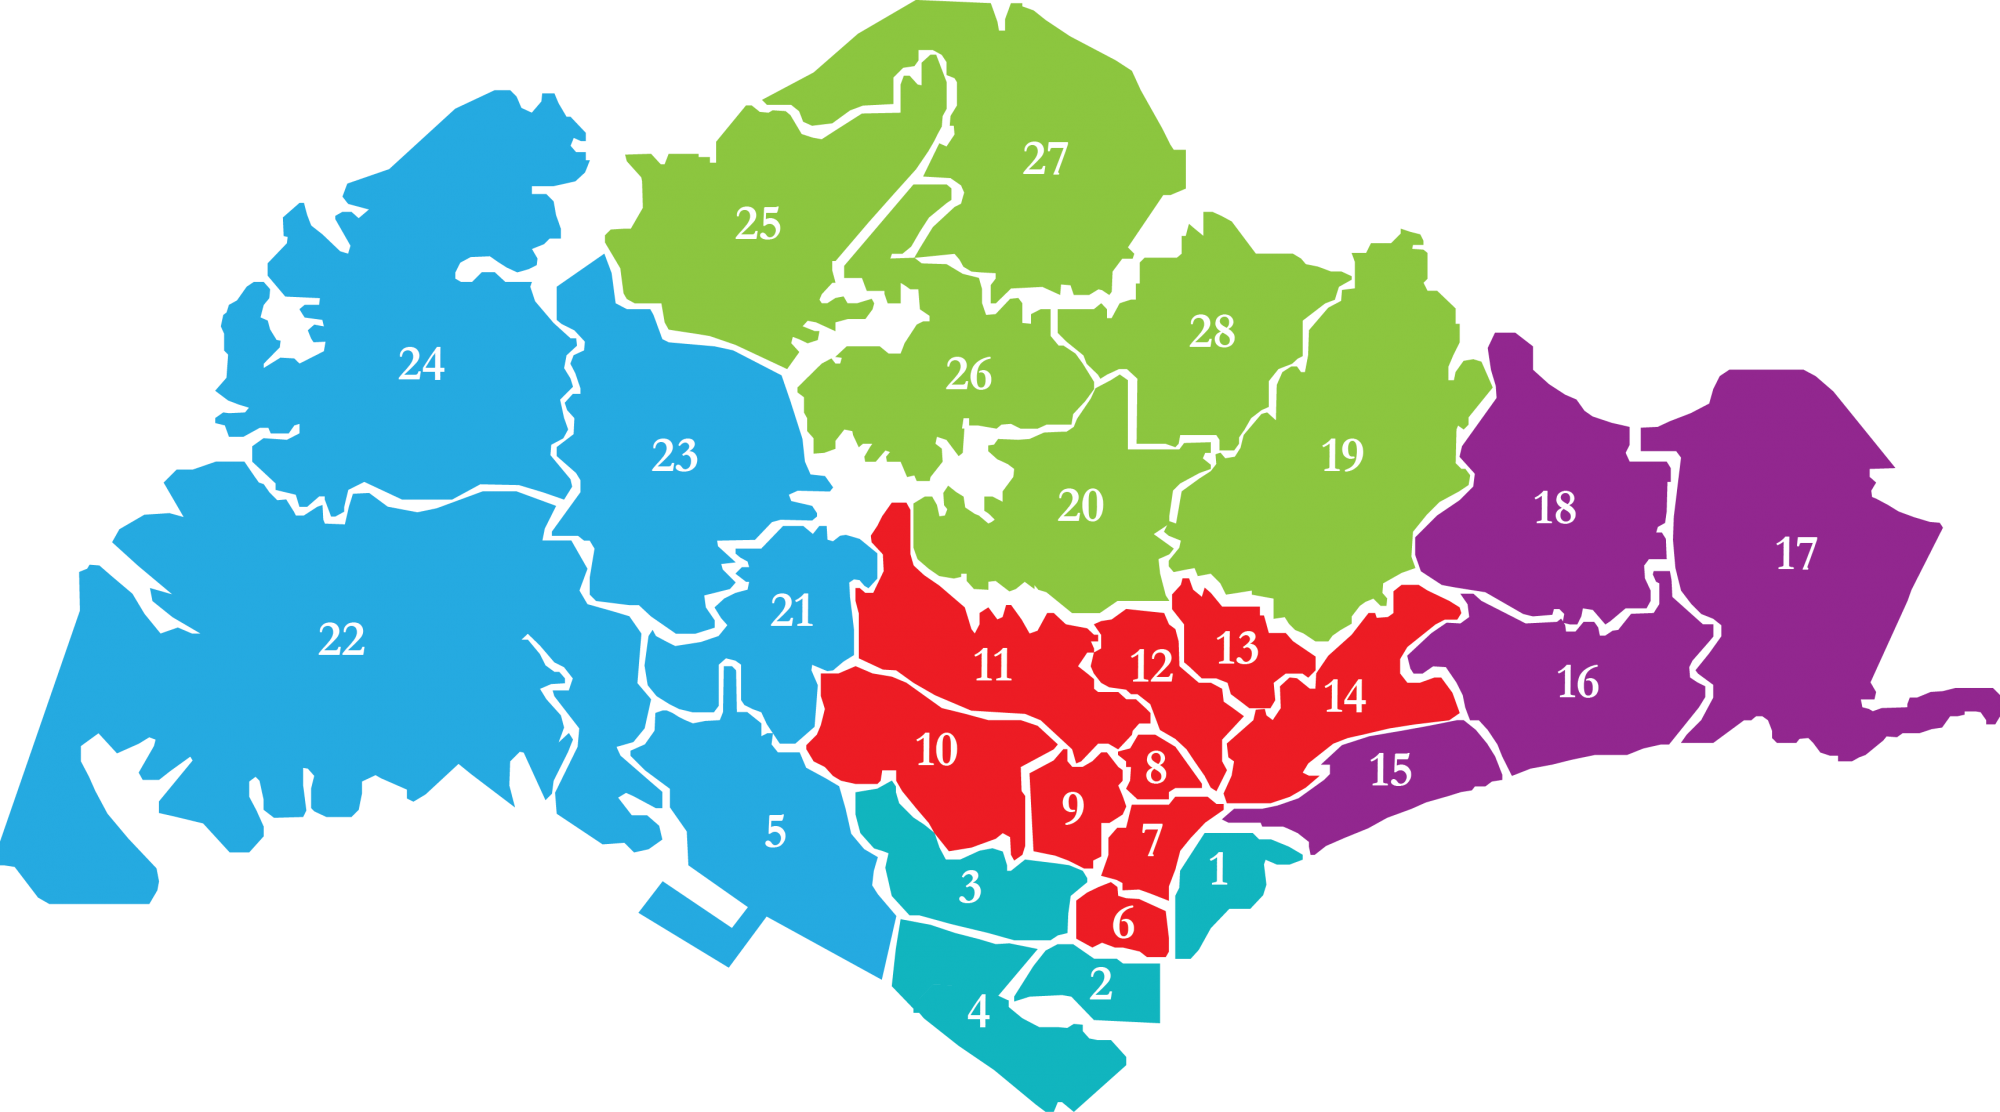
\includegraphics{IMG/img16.png}

Regardless of facilities, people do have preferences on which
estate/town they want to live at. It could be due to their childhood,
proximity to parents and relatives, school admission of the children,
commute to work, etc are some of the common reasons. The behaviour and
frequent transactions drive the prices of HDBs in certain estates higher
than the others.

We extracted the raw transaction data of HDBs from 2019 and analysed the
pricing behaviour by towns, flat type and even remaining years of lease.
The idea of an application for users to provide a one-stop solution to
visually review the transaction history and quickly view the trend by
various factors is motivating for us. An application such as this would
be beneficial to our users who want a consolidated view of the market
history.

\hypertarget{literature-review}{%
\section{Literature Review}\label{literature-review}}

\hypertarget{srx-website}{%
\subsection{SRX Website}\label{srx-website}}

\begin{enumerate}
\def\labelenumi{\arabic{enumi}.}
\tightlist
\item
  Whie performing research on the property of Singapore, we came across
  application from SRX -- a property sale site. There is an application
  within the website to show the pricing trend. The chart is visually
  not very attractive and has many missing components that would benefit
  the users.
\end{enumerate}

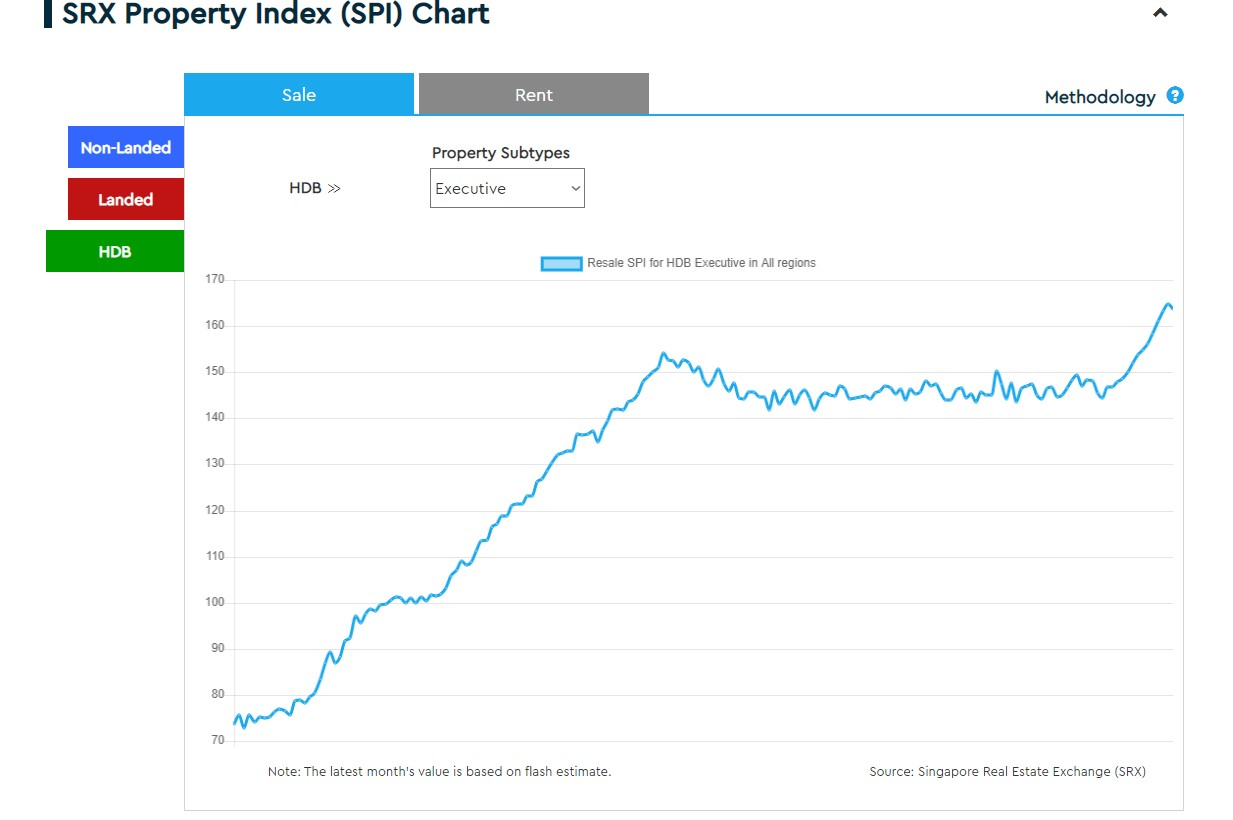
\includegraphics{IMG/img1.jpg} \#\#\# Clarity \& Aesthetic Issues • The
chart is a timeline graph, but it has no time stated in the X axis. One
cannot tell if the chart is for a certain period.

• The selection is only by HDB, Landed and non-Landed. There is no
further segregation by size and, flat type. The absolute \$ variation by
flat type would vary. Hence, it is not good to aggregate the values as a
single line graph.

• Finally, there is no mention of town or estate in the graph. A price
variance in downtown may not be equivalent to the price variance in
suburbs. Multiple factors affect the trend and that must be considered
before dwelling into the pricing trend.

• Overall, the graph is not impressive, and it fails to tell any story
to the user. Website (\url{https://www.srx.com.sg/price-index\#})

\hypertarget{hdb-website}{%
\subsection{HDB website:}\label{hdb-website}}

There are 2 links within the HDB site to provide the resale transactions
of the HDBs within the last 2 years. They are a data table which a user
can retrieve only by keying in exact specific details (down to the
street level) and a geospatial map that provides further insights on
amenities (a search function by street level).
(\url{https://services2.hdb.gov.sg/webapp/BB33RTIS/BB33PReslTrans.jsp})
(\url{https://services2.hdb.gov.sg/web/fi10/emap.html})

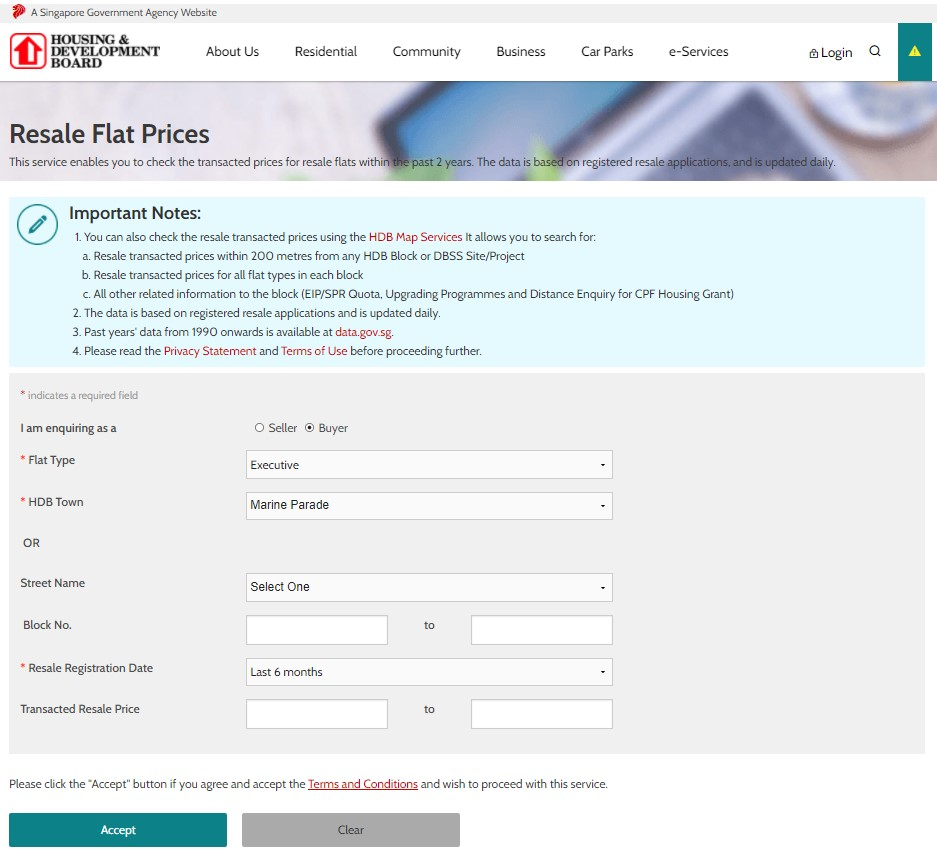
\includegraphics{IMG/img2.jpg}

\hypertarget{clarity-aesthetic-issues}{%
\subsubsection{Clarity \& Aesthetic
Issues}\label{clarity-aesthetic-issues}}

• While HDB website is the most authentic source of data, it does not
provide any visual analysis of the resale transactions done in the last
few years.

• There are no trend lines / graphs for users to compare prices in a
single interactive dashboard.

• There are no searches available as a consolidated view for users to
use the function to compare and understand the trends.

• There are generic guidelines on flat types and sizes but no trends to
show the pricing variance of flat types in various estates.

• These are important considerations that one makes while purchasing
their first home. These must be catered to for a user-friendly
experience.

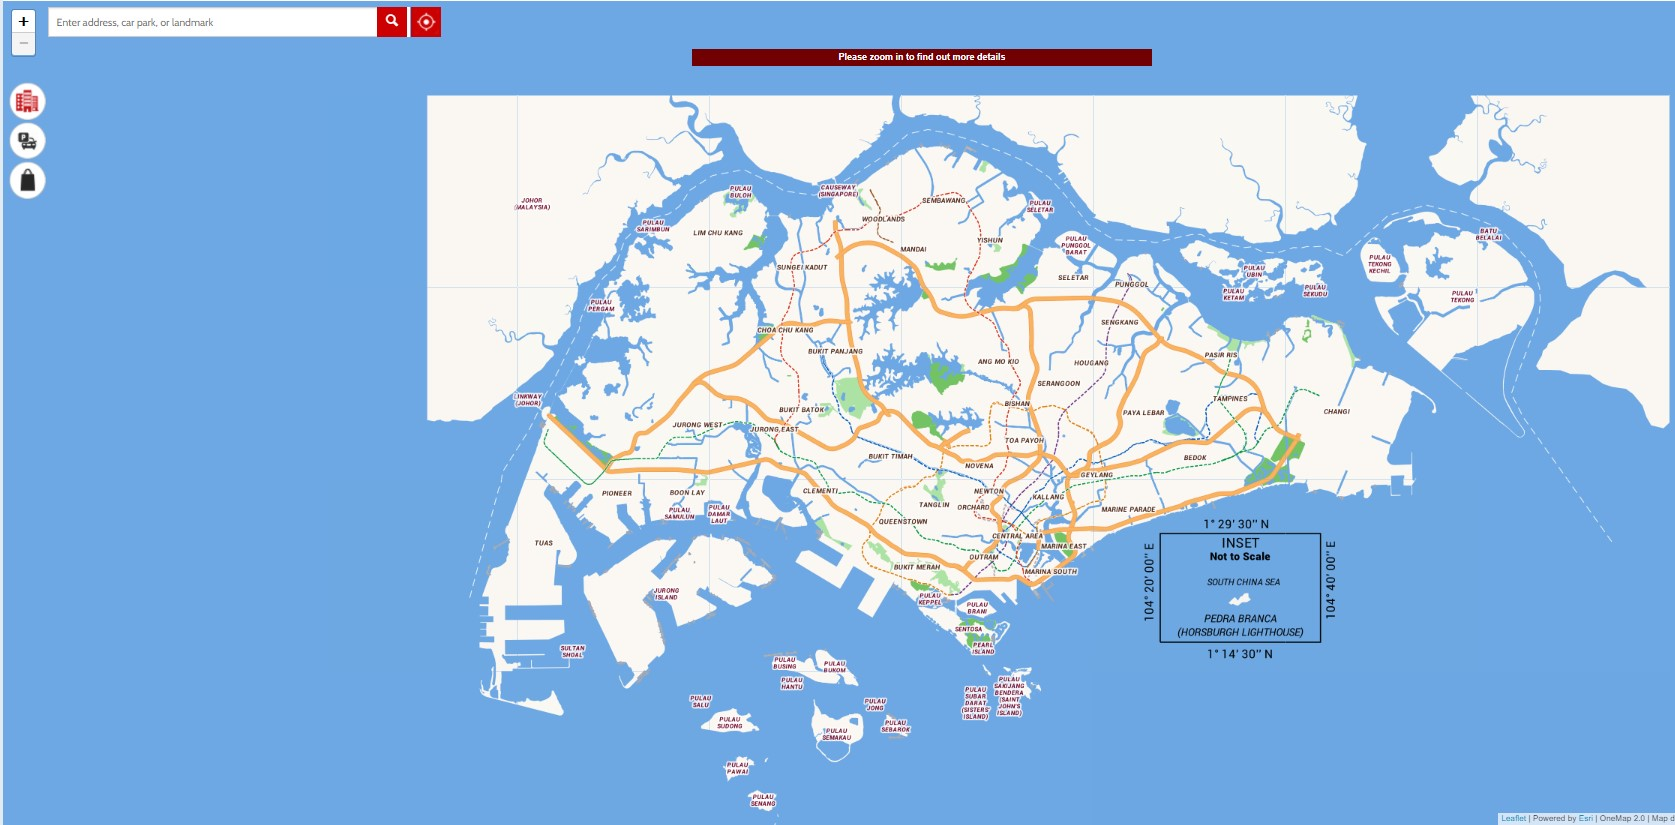
\includegraphics{IMG/img3.jpg}

\hypertarget{data-analysis-methodology}{%
\section{Data Analysis Methodology}\label{data-analysis-methodology}}

\hypertarget{the-planning}{%
\subsection{The Planning}\label{the-planning}}

We decided to approach a 6-step strategy for performing the property
pricing analysis. The steps would span right from data extraction to the
final insights we obtain based on the data analysis performed. The 6
steps would consist of:

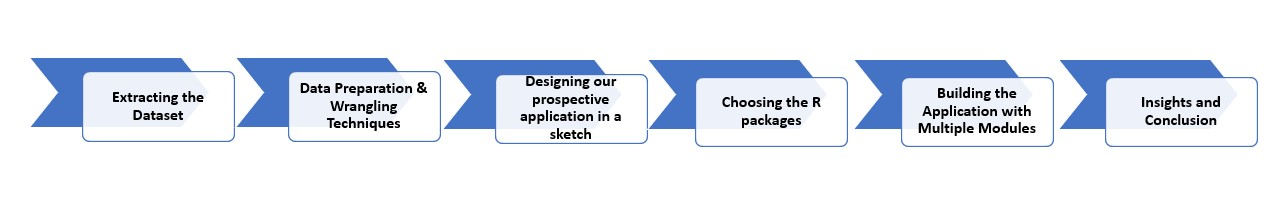
\includegraphics{IMG/img4.jpg}

\hypertarget{data-extraction}{%
\subsection{Data Extraction}\label{data-extraction}}

Data was extracted from Singapore Government's Public Data Website
(\url{https://data.gov.sg/dataset/resale-flat-prices}). This is a
reliable and authentic government website source.

The data consisted of resale prices from 1990 onwards till July 2021.
However, data is very fluid, and we are only interested in years from
2019 Jan till 2021 Jul.~Reason being, property prices are like stocks.
They change radically given a change in circumstance. We are keen to
observe how the prices were pre-Covid, during Covid and almost-post
Covid with high vaccination rates. With projects getting delayed (due to
shortage of labour), many resale HDB prices went up. We do not know how
the pricing will be in future, but we can provide the trend from 2019
(pre-Covid) to show the users how the resale market was.

\hypertarget{data-preparation-and-wrangling}{%
\subsection{Data Preparation and
Wrangling}\label{data-preparation-and-wrangling}}

We used \emph{dplyr package} to filter the data. This gave us data from
2019 onwards. We further used \emph{tidyverse, lubridate and clock
packages} to wrangle the data and bring them to a usable format. We did
not aggregate any of the transactions as we wanted to use the actual
individual transactions for the analysis.

\hypertarget{data-analysis-steps}{%
\subsection{Data Analysis Steps}\label{data-analysis-steps}}

Using Shiny Package in R, we built a holistic application for users to
navigate through various town and browse the property pricing. We built
3 modules in the application.

\hypertarget{geo-facet-mapping}{%
\subsubsection{Geo-Facet Mapping}\label{geo-facet-mapping}}

Using \emph{Geofacet Package} in R, we built 2 visuals: Geofacet of
transaction volumes by town and Geofacet of average pricing by town.
Geofacet is useful here because it provides a flexible way to visualise
data for different geographic locations in Singapore and compare the
results. Visually, this is attractive as it plots itself like the
overall topology of the country.

Geofact is helpful because a user can identify which estates have higher
transaction volumes (possibly due to large estate size or even due to
high demand of housing in the estate). The Geofacet of average pricing
would enable a user to narrow down the list of estates where he/she
wants to further drill down to analyse the trend further. Geofacet has
been built in the form of the Singapore map with individual line graphs
within the town.

\hypertarget{resale-pricing-analysis-by-transaction-volume}{%
\subsubsection{Resale Pricing Analysis by Transaction
Volume}\label{resale-pricing-analysis-by-transaction-volume}}

Using \emph{Plotly package} in R, we built a simple chart to showcase
the transaction volume with average resale pricing. This is an
interactive chart whereby the user can filter by year, by flat type and
town to see the trend. This is useful because it provides a trend over
time on how the resale market worked.

\hypertarget{resale-pricing-analysis-by-flat-type-boxplot}{%
\subsubsection{Resale Pricing Analysis by Flat-Type
(Boxplot)}\label{resale-pricing-analysis-by-flat-type-boxplot}}

Using the \emph{plotly package}, we built box plots for all towns using
the flat-type as a base to determine the mean and median pricing of the
flats across towns. Users can check for outlier transactions using this
chart and check for towns where transactions are higher/lower depending
on their needs.

\hypertarget{interactive-dashboard-let-the-user-choose}{%
\subsubsection{Interactive Dashboard -- Let the User
Choose}\label{interactive-dashboard-let-the-user-choose}}

The final module used in the application is the interactive dashboard
that allows users to choose the factors by town and perform a deep dive
analysis. This is important after the first 2 modules whereby an overall
comparison of towns is shown. Once the user narrows down his list of
towns, he can deep dive further by selecting the town and other factors.
This dashboard is the unique selling point of our application. The
module is built using a combination of packages such as \emph{plotly},
\emph{ggplotly}, \emph{zoo}.

\hypertarget{insights-and-next-steps}{%
\section{Insights and Next Steps}\label{insights-and-next-steps}}

Based on the initial analysis performed, it did seem like the property
prices have increased in the last 2 years. There could be multiple
factors which constitute to the change. Since our resale data does not
have the information, we will refrain from providing further comments on
the change. As a next step, we would like to extract inflation, stock
exchange index, and perform statistical analysis to understand the
correlation between property prices and the economic indicators.

Based on the dashboard, below are some of the outputs of the charts
performed for 2021. This is to show how the market is moving this year.

\hypertarget{geofacet-charts-review}{%
\subsection{Geofacet Charts Review:}\label{geofacet-charts-review}}

It is interesting to note that 4 room flats in Seng Kang and Punggol
have had the highest transaction volumes and are increasing. It could be
due to the launch of BTO flats a few years ago making them available for
resale in the last 2 years. There are many factors here if we look
closely.

• The remaining years of lease is quite high suggesting fast purchase
and sale of flats

• They are steadily increasing since 2019 to 2021.

• Despite high transaction volumes, the average pricing is not the
highest in these estates.

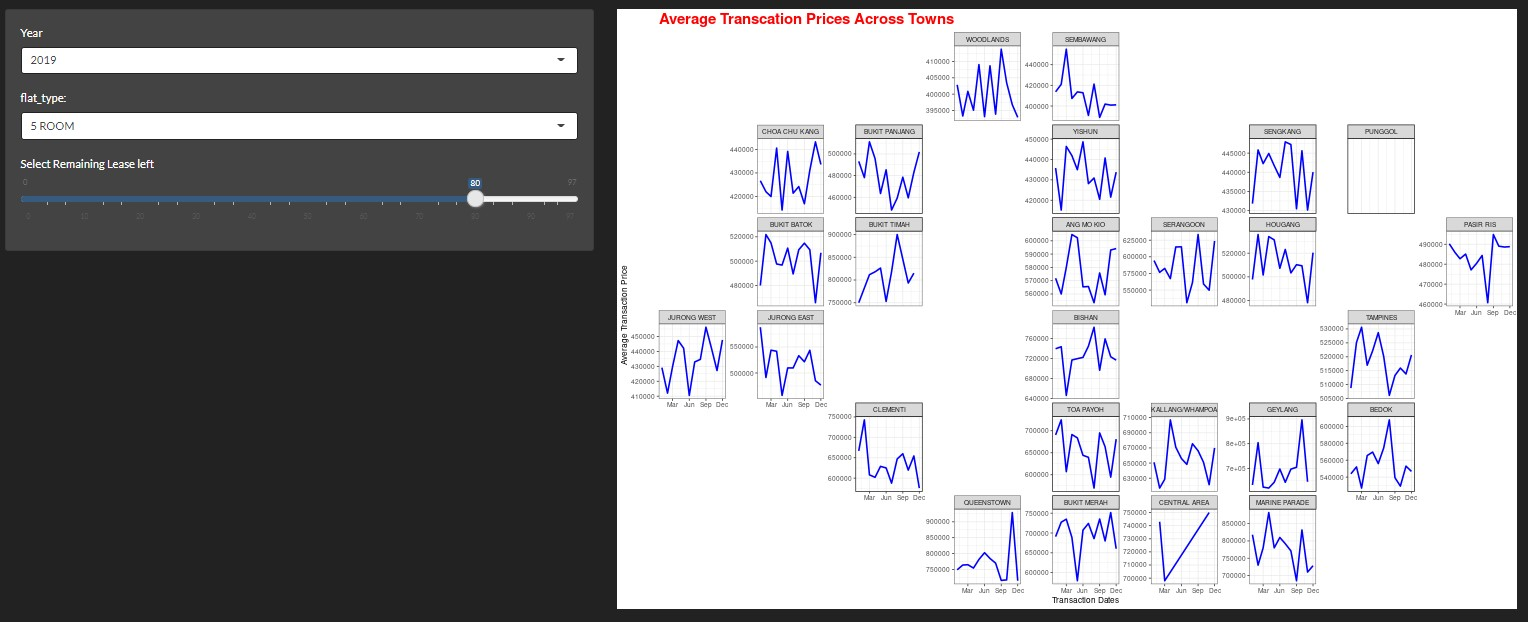
\includegraphics{IMG/img11.jpg}

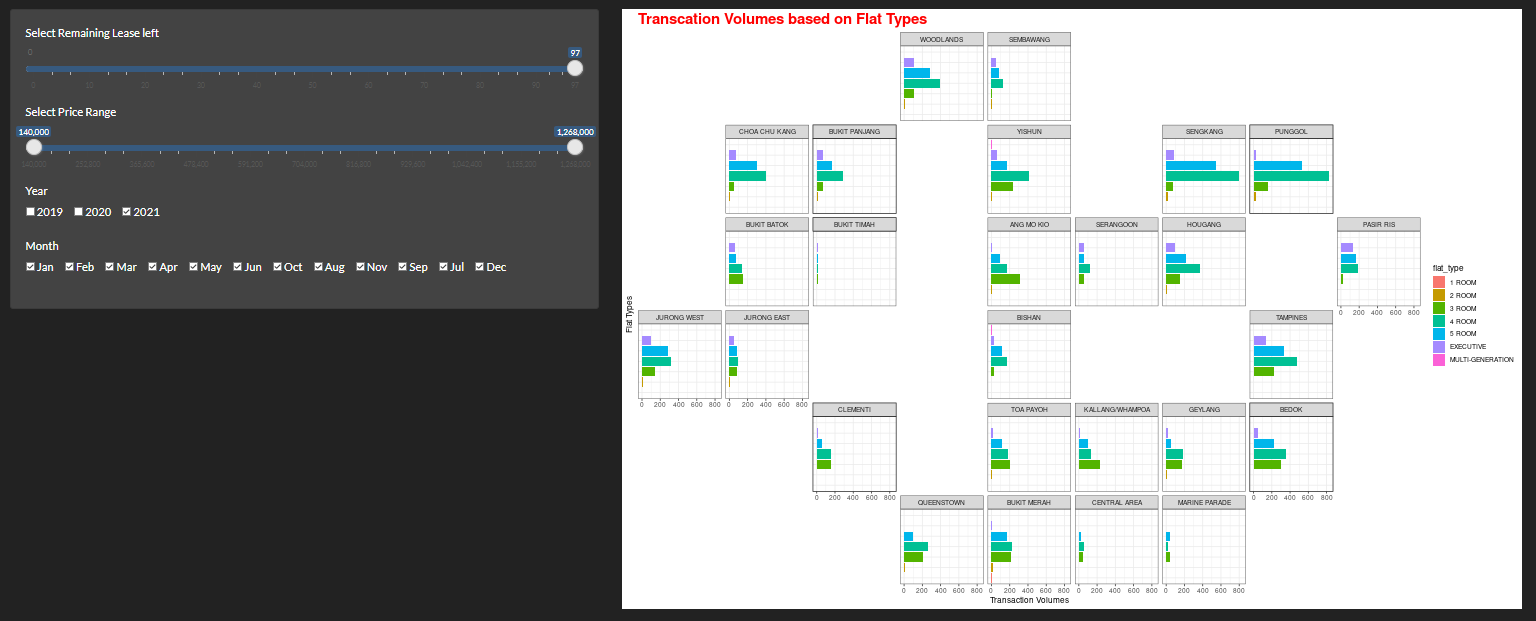
\includegraphics{IMG/img12.png}

\hypertarget{transaction-volumes-vs-average-pricing-review}{%
\subsection{Transaction Volumes vs Average Pricing
Review:}\label{transaction-volumes-vs-average-pricing-review}}

Once we use the Geo-Facet charts to observe the trend of different
estates, we may navigate to the Transaction Volume tab to understand the
trend of the shortlisted estates. Transaction volumes showed an upwards
trend in 2021 Q2. However, by deep-diving into respective estates, we
would know the trend for that estate. In certain estates, the
transactions may be high and possibly due to sudden demand of housing in
the area. That does not necessarily translate to high pricing. Pricing
has many other driving factors such as distance from downtown, type of
flats, size of flats, built year, etc.

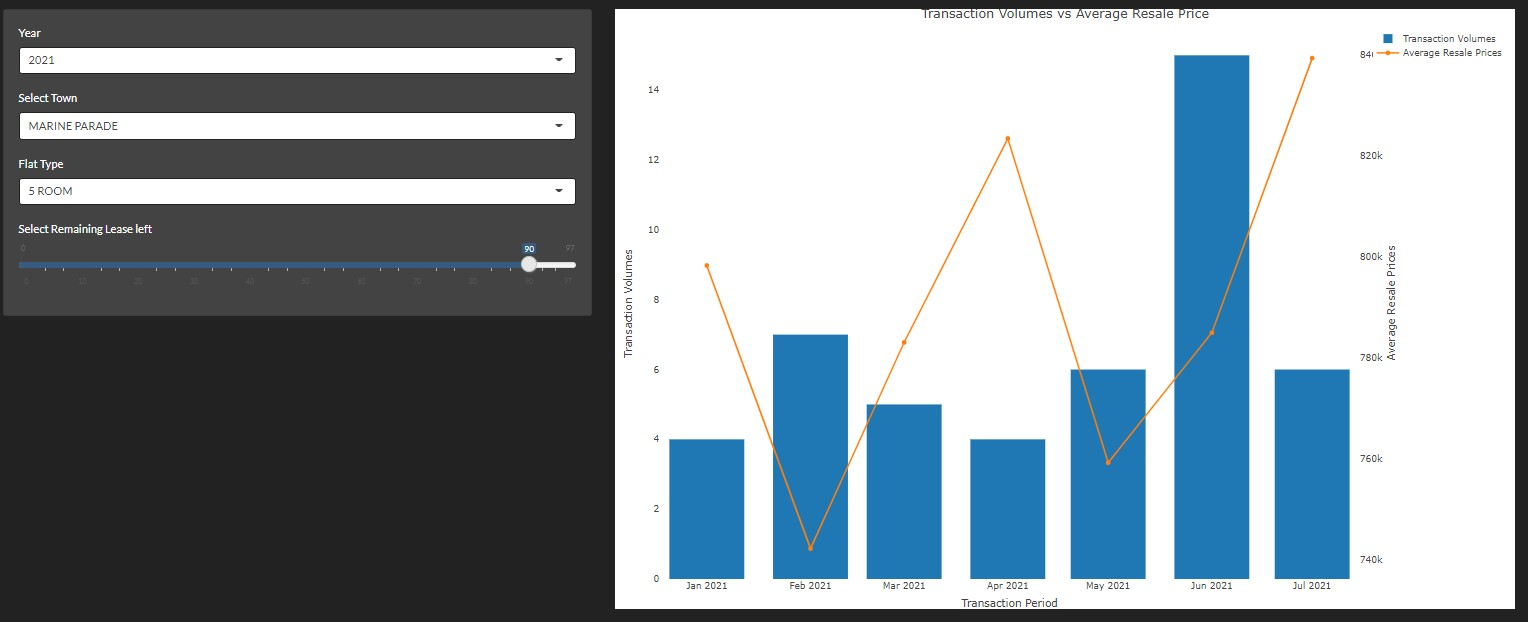
\includegraphics{IMG/img13.jpg}

\hypertarget{resale-price-analyser}{%
\subsection{Resale Price Analyser}\label{resale-price-analyser}}

Once we use the transaction volume analyser to understand how the
pricing moves for different estates in relation to volumes, we may want
to deep dive further to understand the mean and median pricing in these
shortlisted estates. This is an important indicator to identify if the
pricing is stable (with low std deviation) or the range is wide with
many outliers. Users can therefore choose estates which are stable or
volatile based on their investment or housing needs.

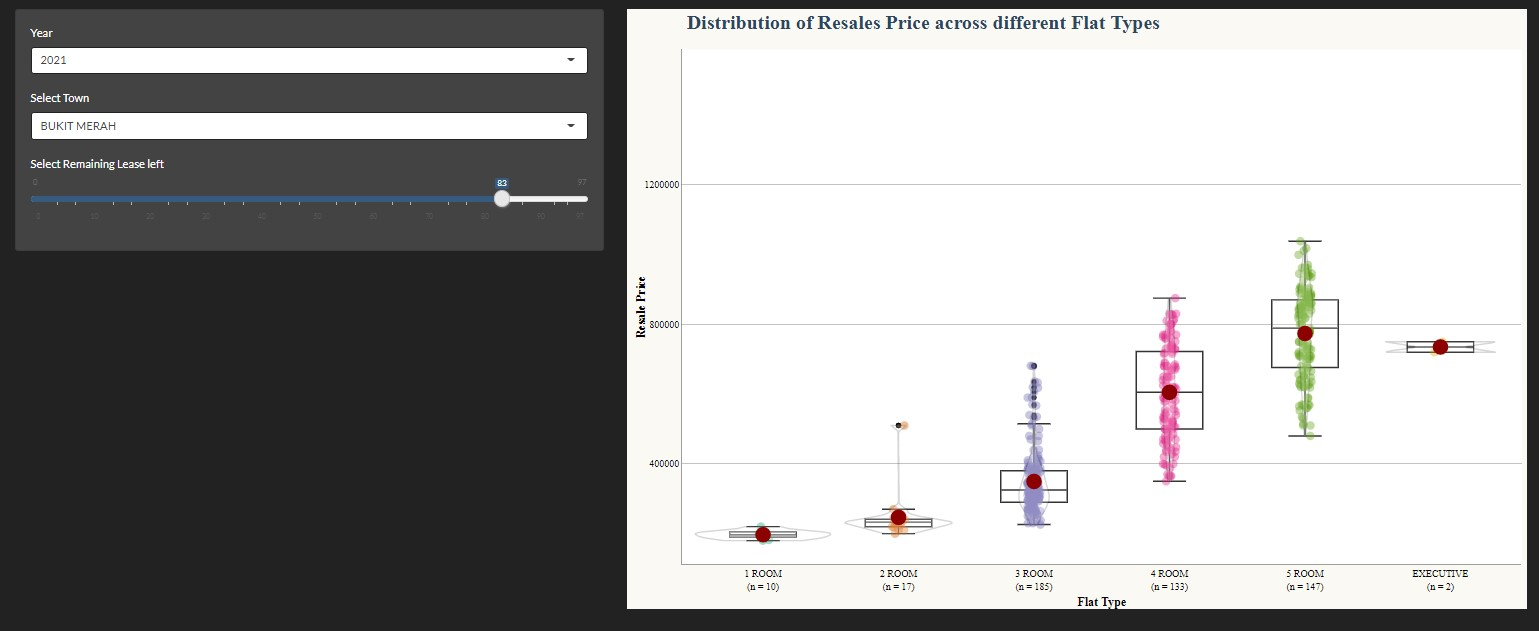
\includegraphics{IMG/img14.jpg}

\hypertarget{all-attributes-review-by-town}{%
\subsection{All Attributes Review by
Town:}\label{all-attributes-review-by-town}}

Upon reviewing and shortlisting the top few town choices, a natural
action a buyer or seller would take is to view the detailed transaction
prices based on his/her choice of flat. The below is an example of how
the data search table would look like for a buyer with an intention to
purchase an executive flat in Punggol with a high remaining year of
lease. He would want to check all latest transactions up to the latest
month for gaining real time insight. The application would show the user
all results of transactions in Punggol for executive flats from April
till July. A user would be able to select the attributes in this search
table and view all transactions including the size of the flat in psf
and psm terms.

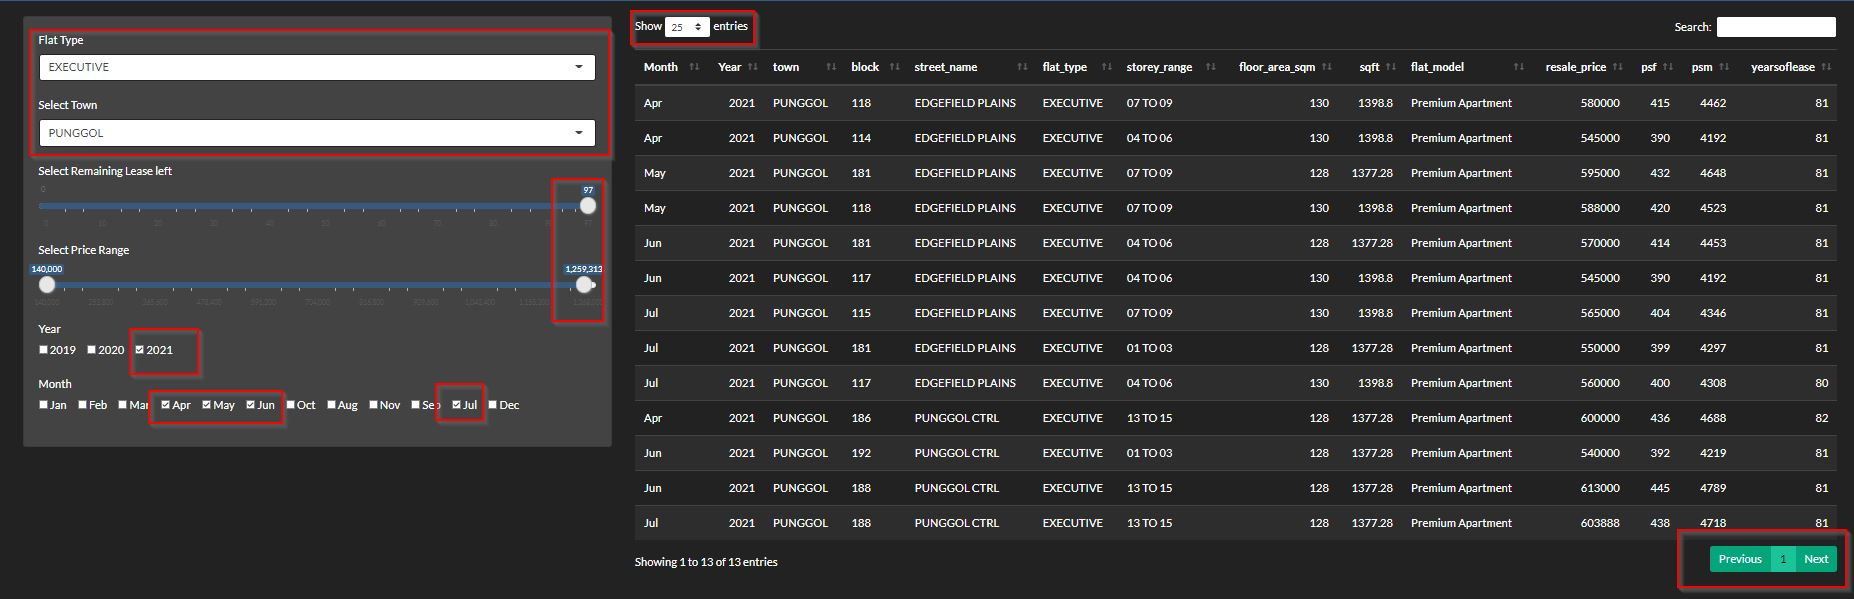
\includegraphics{IMG/img15.jpg}

\hypertarget{the-realis-guru-application}{%
\section{The Realis-Guru
Application}\label{the-realis-guru-application}}

The link to the application is here: RealisGuru
(\url{https://realisguru.shinyapps.io/VAapp/})

\hypertarget{references}{%
\subsection{\# References}\label{references}}

references: - container-title:
\url{https://www.asiaone.com/money/how-hot-singapore-property-market-2021}
author: - given: Stuart type: Website publisher: AsiaOne issued: year:
2021 month: 6 ---

\begin{itemize}
\tightlist
\item
  title: Edge Fair-Value container-title: EdgeProp Fair-Value URL:
  `\url{https://www.edgeprop.sg/analytic/edgefairvalue}' publisher: Edge
  Prop type: Website issued:Web Version 4.5.136 \ldots{}
\end{itemize}

\begin{Shaded}
\begin{Highlighting}[]
\NormalTok{tinytex}\SpecialCharTok{::}\FunctionTok{install\_tinytex}\NormalTok{()}
\end{Highlighting}
\end{Shaded}

\setlength{\parindent}{0in}

\end{document}
